% ============================================================
% Appendix
% ============================================================

\section{KISPE SATLL}
\label{app:satll}

The SATLL's On-Board Data Handling (OBDH) subsystem is based on an STM32H573 microcontroller, which belongs to the same processor family as those used in KISPE's flight on-board computers  \cite{KISPE2025}. This subsystem manages the satellite's command and data handling functions. All subsystems communicate via a shared CAN bus, with the OBDH serving as the central node for collecting telemetry and issuing telecommands. The bus transmits distributed voltage, current, temperature, and status telemetry from all boards, making it the primary data path for both routine operations and potential adversarial activities targeting onboard systems. The IDS is integrated directly into the OBDH software, enabling passive monitoring of the CAN bus without disrupting normal operations.

\begin{figure}
    \centering
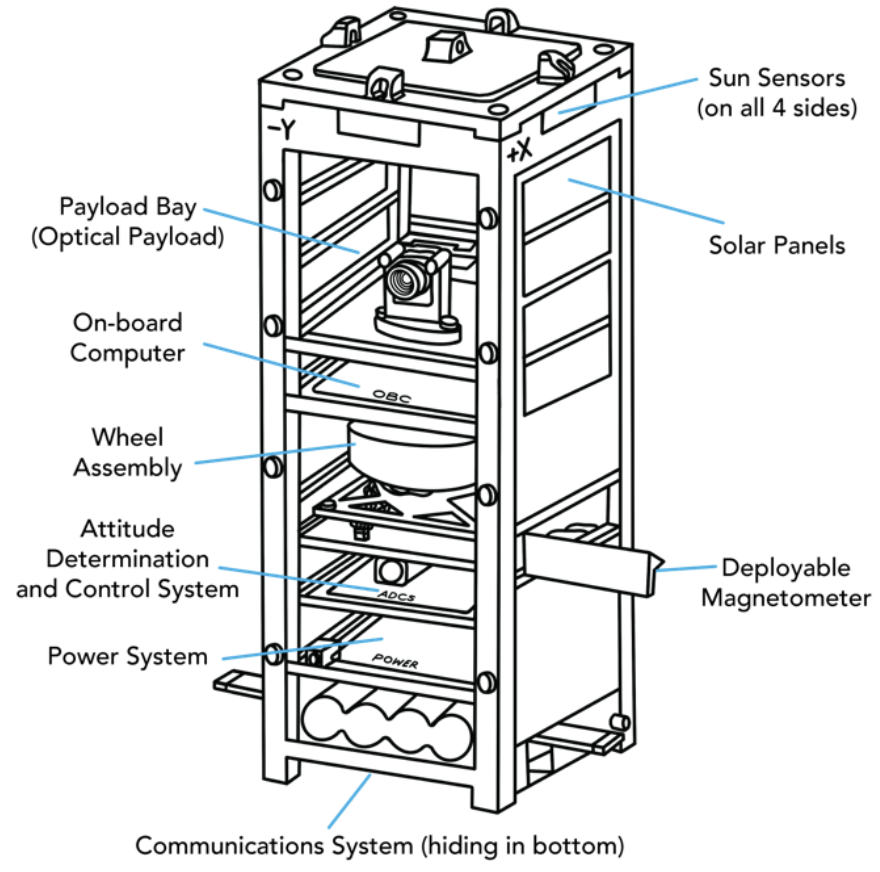
\includegraphics[width=0.75\linewidth]{images/SatDiagram.png}
    \caption{KISPE Satellite Learning Laboratory (SATLL) Diagram}
    \label{fig:diagram}
\end{figure}


\section{CAN Feature Extraction Algorithm}
\label{app:feature_extraction}

Algorithm~\ref{alg:features} gives the pseudocode for the sliding-window CAN feature extractor (implemented in \texttt{can\_feature\_engineering.py}). The extractor maintains per-ID rolling history and a global window deque of the most recent $W=50$ frames. All per-frame quantities are computed in $O(1)$ time; window statistics require one pass over the deque on each new frame, bounded by $O(W)$.

\begin{algorithm}[H]
\caption{CAN Sliding-Window Feature Extraction}
\label{alg:features}
\begin{algorithmic}[1]
\Require CAN frame stream $\mathcal{F}$; baseline $\mathcal{B}$: ID $\to$ expected DLC; window size $W$
\Ensure Per-frame feature vector $\mathbf{x} \in \mathbb{R}^{14}$ and label $y$
\State $\textit{window} \leftarrow$ empty deque (capacity $W$)
\State $\textit{prev}[\cdot] \leftarrow \emptyset$ \Comment{last frame per CAN ID}
\State $\textit{arrival}[\cdot] \leftarrow []$ \Comment{timestamp history per CAN ID}
\For{each frame $f = (\tau, \textit{id}, \textit{dlc}, \mathbf{d}, y)$}
    \State Append $f$ to $\textit{window}$; evict oldest if $|\textit{window}| > W$
    \State $\mathbf{p} \leftarrow \textit{prev}[\textit{id}]$ (or zeros if unseen)
    \State \textbf{// Payload structure}
    \State $x_1 \leftarrow \textit{id} / 2047$ \Comment{\texttt{can\_id\_norm}}
    \State $x_2 \leftarrow \textit{dlc}$
    \State $x_3 \leftarrow \mathrm{mean}(\mathbf{d})$;\; $x_4 \leftarrow \mathrm{std}(\mathbf{d})$
    \State $x_5 \leftarrow H(\mathbf{d})$ \Comment{Shannon entropy, bits}
    \State $x_6 \leftarrow \max(\mathbf{d}) - \min(\mathbf{d})$
    \State $x_7 \leftarrow \mathrm{popcount}(\mathbf{d} \oplus \mathbf{p}.\mathbf{d})$ \Comment{Hamming distance}
    \State $x_8 \leftarrow \sum_i |\mathbf{d}_i - \mathbf{p}.\mathbf{d}_i|$ \Comment{L1 payload delta}
    \State $x_9 \leftarrow \mathbf{1}[\textit{dlc} \neq \mathcal{B}[\textit{id}]]$ \Comment{\texttt{dlc\_anomaly}}
    \State $x_{10} \leftarrow \mathbf{1}[\textit{id} \in \mathcal{B}]$ \Comment{\texttt{id\_is\_known}}
    \State \textbf{// Temporal dynamics} (over \textit{window})
    \State $\Delta \leftarrow$ inter-arrival times of \textit{id} within \textit{window}
    \State $x_{11} \leftarrow \mathrm{mean}(\Delta)$
    \State $x_{12} \leftarrow |\{f' \in \textit{window} : f'.\textit{id} = \textit{id}\}| \;/\; (\textit{window\_span})$
    \State \textbf{// Bus topology} (over \textit{window})
    \State $x_{13} \leftarrow |\textit{window}| \;/\; (\textit{window\_span})$ \Comment{\texttt{bus\_load}}
    \State $x_{14} \leftarrow |\{\,f'.\textit{id} : f' \in \textit{window}\}|$ \Comment{\texttt{unique\_ids}}
    \State \textbf{yield} $(\mathbf{x}, y)$
    \State $\textit{prev}[\textit{id}] \leftarrow f$
\EndFor
\end{algorithmic}
\end{algorithm}


\begin{table}[t]
\caption{CAN IDS feature set (14 total). ``Window'' features are computed over the offline 50-frame sliding history; ``per-frame'' features are computed from the current frame and its same-ID predecessor.}
\label{tab:features}
\small
\begin{tabular}{@{}lp{5.2cm}@{}}
\toprule
\textbf{Feature} & \textbf{Description} \\
\midrule
\multicolumn{2}{@{}l}{\textit{Payload structure (per-frame)}} \\
\texttt{data\_mean}    & Mean of 8 payload bytes \\
\texttt{data\_std}     & Std.\ dev.\ of payload bytes \\
\texttt{data\_entropy} & Shannon entropy of payload \\
\texttt{data\_range}   & max$-$min of payload bytes \\
\texttt{dlc}           & Data length code (0--8) \\
\texttt{dlc\_anomaly}  & 1 if DLC deviates from trained baseline \\
\texttt{hamming\_dist} & Bit Hamming distance from previous same-ID frame \\
\texttt{payload\_delta}& L1 distance from previous same-ID payload \\
\midrule
\multicolumn{2}{@{}l}{\textit{Temporal dynamics (window)}} \\
\texttt{inter\_arrival\_mean} & Mean $\Delta t$ between same-ID frames \\
\texttt{id\_freq}             & This ID's message rate (msgs/s) \\
\texttt{bus\_load}            & Total bus message rate (msgs/s) \\
\midrule
\multicolumn{2}{@{}l}{\textit{Bus topology (window)}} \\
\texttt{can\_id\_norm} & Normalized 11-bit arbitration ID \\
\texttt{unique\_ids}   & Distinct IDs observed in window \\
\texttt{id\_is\_known} & 1 if this ID was seen during training \\
\bottomrule
\end{tabular}
\end{table}

% ============================================================
\section{Inference Algorithm}
\label{app:inference}

Algorithm~\ref{alg:inference} describes the onboard inference path executed by the STM32 firmware. The entire computation is stack-allocated; no heap calls occur. The feature buffer \texttt{feat[14]} (56~bytes) is populated by the CAN ISR or polling loop; \texttt{scale()} applies the precomputed z-score constants stored in flash; \texttt{tree\_predict()} traverses the 39-node decision tree using the exported C arrays.

\begin{algorithm}[t]
\caption{CAN IDS Inference (STM32)}
\label{alg:inference}
\begin{algorithmic}[1]
\Require CAN frame $f$; static flash arrays: \texttt{thresholds[N]}, \texttt{feature\_idx[N]},
         \texttt{children\_left[N]}, \texttt{children\_right[N]}, \texttt{leaf\_class[N]};
         static scaler arrays: \texttt{mean[14]}, \texttt{scale[14]}
\Ensure Alert flag $\hat{y} \in \{0,1\}$; clock cycles elapsed
\State \textbf{// Feature computation (CAN ISR context)}
\State \texttt{feat[14]} $\leftarrow$ \Call{compute\_features}{$f$, \textit{window}, \textit{baseline}}
\State \textbf{// Z-score normalization}
\For{$i \leftarrow 0$ \textbf{to} $13$}
    \State \texttt{feat[i]} $\leftarrow$ (\texttt{feat[i]} $-$ \texttt{mean[i]}) $/$ \texttt{scale[i]}
\EndFor
\State \textbf{// Tree traversal}
\State $\textit{node} \leftarrow 0$
\While{\texttt{children\_left[node]} $\neq -1$}  \Comment{not a leaf}
    \If{\texttt{feat[feature\_idx[node]]} $\leq$ \texttt{thresholds[node]}}
        \State $\textit{node} \leftarrow$ \texttt{children\_left[node]}
    \Else
        \State $\textit{node} \leftarrow$ \texttt{children\_right[node]}
    \EndIf
\EndWhile
\State $\hat{y} \leftarrow$ \texttt{leaf\_class[node]}
\If{$\hat{y} = 1$}
    \State \Call{ids\_raise\_alert}{$f$.\textit{id}, $\tau$} \Comment{publish via telemetry}
\EndIf
\State \Return $\hat{y}$
\end{algorithmic}
\end{algorithm}

% ============================================================
\section{Benchmark-to-CAN Encoding Algorithm}
\label{app:b2can}

Algorithm~\ref{alg:b2can} formalizes the tabular-to-CAN encoding used in the cross-domain experiment (Section~\ref{sec:methodology}). Each tabular sample of $F$ features is serialized as $1 + \lceil F/8 \rceil$ CAN frames: one meta frame carrying the sample index and binary label, followed by payload frames carrying min-max-scaled uint8 feature values packed 8 bytes at a time.

\begin{algorithm}[t]
\caption{Tabular-to-CAN Frame Encoding}
\label{alg:b2can}
\begin{algorithmic}[1]
\Require Tabular dataset $\{(\mathbf{x}_i, y_i)\}_{i=1}^{N}$; dataset code $c \in \{1,2\}$;
         inter-frame gap $\delta t = 1$~ms; meta CAN ID $\textit{id}_m$; base payload ID $\textit{id}_b$
\Ensure CAN frame stream with columns [\textit{timestamp}, \textit{can\_id}, \textit{dlc}, $d_0\ldots d_7$, \textit{label}]
\State $\mathbf{a} \leftarrow \min_i(\mathbf{x}_i)$;\; $\mathbf{b} \leftarrow \max_i(\mathbf{x}_i)$ \Comment{fit scaler on train split only}
\State $\tau \leftarrow 0$
\For{$i \leftarrow 1$ \textbf{to} $N$}
    \State $\mathbf{u} \leftarrow \mathrm{clip}\!\left(\left\lfloor 255 \cdot \tfrac{\mathbf{x}_i - \mathbf{a}}{\mathbf{b} - \mathbf{a}} \right\rceil,\, 0,\, 255\right)$ \Comment{uint8 encoding}
    \State \textbf{emit} meta frame: $(\tau,\; \textit{id}_m,\; 8,\;
           [i_{\&},\, i_{\gg 8},\, i_{\gg 16},\, y_i,\, \lceil F/8\rceil,\, c,\, \textit{split},\, 0])$
    \State $\tau \leftarrow \tau + \delta t$
    \For{$k \leftarrow 0$ \textbf{to} $\lceil F/8 \rceil - 1$}
        \State $\textit{chunk} \leftarrow \mathbf{u}[8k : \min(8k+8, F)]$ (zero-padded to 8 bytes)
        \State $\textit{dlc}   \leftarrow \min(8,\; F - 8k)$
        \State \textbf{emit} $(\tau,\; \textit{id}_b + k,\; \textit{dlc},\; \textit{chunk},\; y_i)$
        \State $\tau \leftarrow \tau + \delta t$
    \EndFor
\EndFor
\end{algorithmic}
\end{algorithm}

% ============================================================
\section{Feature Mathematical Definitions}
\label{app:feature_math}

Table~\ref{tab:feature_math} gives the precise mathematical definition of each of the 14 CAN features. $\mathcal{W}(t)$ denotes the set of frames in the sliding window at time $t$; $\mathcal{W}_{\textit{id}}(t)$ is the subset with matching arbitration ID. $\mathbf{d}(f)$ denotes the 8-byte payload vector of frame $f$; $\tau(f)$ its timestamp.

\begin{table}[t]
\caption{Mathematical definitions of the 14 CAN IDS features. $n = |\mathbf{d}|$; $H(\cdot)$ is Shannon entropy (bits); $W = |\mathcal{W}(t)|$.}
\label{tab:feature_math}
\small
\begin{tabular}{@{}ll@{}}
\toprule
\textbf{Feature} & \textbf{Definition} \\
\midrule
\texttt{can\_id\_norm}        & $\textit{id}\;/\;2047$ \\
\texttt{dlc}                  & $\textit{dlc}(f)$ \\
\texttt{data\_mean}           & $\frac{1}{n}\sum_i d_i$ \\
\texttt{data\_std}            & $\sqrt{\frac{1}{n}\sum_i(d_i - \bar{d})^2}$ \\
\texttt{data\_entropy}        & $H(\mathbf{d}) = -\sum_v p_v \log_2 p_v$ \\
\texttt{data\_range}          & $\max(\mathbf{d}) - \min(\mathbf{d})$ \\
\texttt{hamming\_dist}        & $\|\mathbf{d}(f) \oplus \mathbf{d}(f_{\textit{prev}})\|_{\mathrm{H}}$ \\
\texttt{payload\_delta}       & $\|\mathbf{d}(f) - \mathbf{d}(f_{\textit{prev}})\|_1$ \\
\texttt{dlc\_anomaly}         & $\mathbf{1}[\textit{dlc}(f) \neq \mathcal{B}[\textit{id}]]$ \\
\texttt{id\_is\_known}        & $\mathbf{1}[\textit{id} \in \mathcal{B}]$ \\
\texttt{inter\_arrival\_mean} & $\frac{1}{|\mathcal{W}_{\textit{id}}|-1}\sum \Delta\tau_{\textit{id}}$ \\
\texttt{id\_freq}             & $|\mathcal{W}_{\textit{id}}(t)|\;/\;\Delta\tau_{\mathcal{W}}$ \\
\texttt{bus\_load}            & $W\;/\;\Delta\tau_{\mathcal{W}}$ \\
\texttt{unique\_ids}          & $|\{\textit{id}(f') : f' \in \mathcal{W}(t)\}|$ \\
\bottomrule
\end{tabular}

\smallskip\footnotesize{$\Delta\tau_{\mathcal{W}} = \tau(f_{\text{newest}}) - \tau(f_{\text{oldest}})$ in window.}
\end{table}

% ============================================================
\section{Per-Attack-Type Detection Results}
\label{app:per_attack}

Table~\ref{tab:per_attack_full} gives per-attack-type recall for all pipeline variants that support per-class breakdown.

\begin{table}[t]
\caption{Per-attack-type recall (\%). Native CAN (Phase~4, $n_\text{test}=5{,}166$): four canonical satellite bus attack classes. NSL$\to$CAN (STM32 hardware, $n=48{,}000$ frames): all 30 attack types in the test split; FPR is a global figure for the configuration. Higher-recall attacks tend to alter payload statistics detectable via entropy/Hamming features.}
\label{tab:per_attack_full}
\small
\begin{tabular}{@{}lrr@{}}
\toprule
\textbf{Attack type} & \textbf{Recall (\%)} & \textbf{FPR (\%)} \\
\midrule
\multicolumn{3}{@{}l}{\textit{Native CAN IDS (Phase~4)}} \\
DoS          & 99.89 & 4.53 \\
Fuzzy        & 99.94 & 4.53 \\
Spoofing     & 100.0 & 4.53 \\
Replay       &  97.78 & 4.53 \\
\midrule
\multicolumn{3}{@{}l}{\textit{NSL$\to$CAN transfer on STM32 hardware}} \\
udpstorm     & 85.71 & 10.76 \\
xlock        & 57.14 & 10.76 \\
rootkit      & 54.76 & 10.76 \\
buffer\_overflow & 52.38 & 10.76 \\
mailbomb     & 45.21 & 10.76 \\
pod          & 41.90 & 10.76 \\
warezmaster  & 37.45 & 10.76 \\
snmpgetattack& 37.20 & 10.76 \\
guess\_passwd& 36.76 & 10.76 \\
ps           & 36.73 & 10.76 \\
processtable & 36.53 & 10.76 \\
smurf        & 36.01 & 10.76 \\
saint        & 35.64 & 10.76 \\
ipsweep      & 37.99 & 10.76 \\
back         & 35.04 & 10.76 \\
mscan        & 35.32 & 10.76 \\
neptune      & 35.24 & 10.76 \\
snmpguess    & 32.80 & 10.76 \\
portsweep    & 35.31 & 10.76 \\
httptunnel   & 31.11 & 10.76 \\
apache2      & 34.41 & 10.76 \\
satan        & 32.16 & 10.76 \\
phf          & 28.57 & 10.76 \\
land         & 28.57 & 10.76 \\
multihop     & 26.19 & 10.76 \\
named        & 25.00 & 10.76 \\
nmap         & 24.84 & 10.76 \\
teardrop     & 20.00 & 10.76 \\
sendmail     &  9.52 & 10.76 \\
xsnoop       &  9.52 & 10.76 \\
xterm        &  7.14 & 10.76 \\
\bottomrule
\end{tabular}
\end{table}

% ============================================================
\section{USB OTG Benchmark Wire Protocol}
\label{app:protocol}

Table~\ref{tab:protocol} documents the binary wire protocol used by \texttt{host\_inference\_runner.py} to drive the STM32 benchmark firmware. All multi-byte integers are little-endian.

\begin{table}[t]
\caption{USB OTG (CDC ACM) binary protocol between host runner and STM32 firmware. Sizes are in bytes.}
\label{tab:protocol}
\small
\begin{tabular}{@{}llrl@{}}
\toprule
\textbf{Direction} & \textbf{Message} & \textbf{Size} & \textbf{Contents} \\
\midrule
Host $\to$ MCU & Start      & 3  & \texttt{'S'} + uint16 $N$ (sample count) \\
Host $\to$ MCU & Features   & 56 & 14 $\times$ float32 feature vector \\
Host $\to$ MCU & Label      & 1  & uint8 ground-truth class (0/1) \\
MCU $\to$ Host & Sample result & 16 & uint8 pred, uint8 gt, uint32 cycles, \\
               &            &    & uint32 stack HWM, uint32 heap free, \\
               &            &    & int32 reserved \\
MCU $\to$ Host & Summary    & 64 & $N$, correct, TP, TN, FP, FN, \\
               &            &    & cyc\_min, cyc\_max, cyc\_sum\_hi, \\
               &            &    & cyc\_sum\_lo, stack\_hwm, energy\_nJ, \\
               &            &    & inf\_us\_mean, acc, prec, rec, f1, fpr \\
               &            &    & (18 fields: 11 $\times$ uint32 + 7 $\times$ float32) \\
\bottomrule
\end{tabular}
\end{table}

The MCU emits \texttt{[IDS]} prefixed log lines over the same USB CDC channel before the binary exchange; the host flushes these before initiating the sample stream. Cycle counts are measured with the ARM DWT cycle counter; stack high-water mark is measured using a canary fill pattern over a 1~KB task-stack region.

% ============================================================
\section{Quantization and Model Export}
\label{app:quantization}

Three numeric precision variants of the trained decision tree are exported as self-contained C headers: Float32 (32-bit IEEE thresholds), Int16 (linearly quantized 16-bit), and Int8 (8-bit). The quantized variants replace floating-point threshold comparisons with integer comparisons, eliminating FPU dependencies and enabling deployment on Cortex-M0 and M0+ cores.

All three formats are evaluated on the UNSW-NB15 test set (82K samples); results are shown in Table~\ref{tab:quant} and Figure~\ref{fig:quant_tradeoffs}. Float32 retains full detection quality (99.43\% recall, 85.24\% F1). Int16 maintains comparable recall (99.32\%) with slightly elevated FPR, at the cost of a 31\% increase in code size due to alignment overhead in the generated header. Int8 degrades markedly: recall falls to 66.4\% and F1 to 65.5\%, indicating that 8-bit precision is insufficient to represent the decision thresholds of a tree trained on z-scored floating-point features without a calibrated quantization pass. All three formats keep the model below 800~bytes, well within the flash budget of any STM32 variant.

\begin{table}[h]
\caption{Quantization comparison on UNSW-NB15 test set (82K samples).}
\label{tab:quant}
\small
\begin{tabular}{@{}lrrrrr@{}}
\toprule
\textbf{Format} & \textbf{Size} & \textbf{Acc.} & \textbf{Rec.} & \textbf{F1} & \textbf{Lat.} \\
                & (bytes)        & (\%)          & (\%)          & (\%)        & (\textmu s)   \\
\midrule
Float32 & 548 & 81.0 & 99.4 & 85.2 & 2.35 \\
Int16   & 731 & 77.0 & 99.3 & 82.6 & 6.32 \\
Int8    & 680 & 61.5 & 66.4 & 65.5 & 6.30 \\
\bottomrule
\end{tabular}
\end{table}

\begin{figure}[h]
  \centering
  \begin{subfigure}[b]{0.48\linewidth}
    \centering
    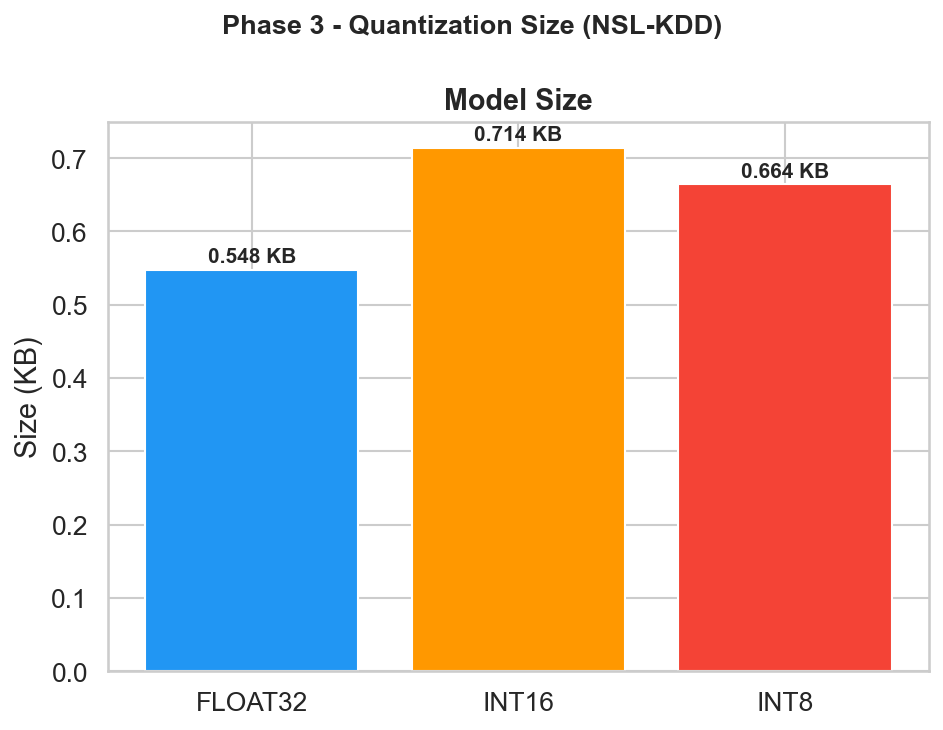
\includegraphics[width=\linewidth]{images/06b_quantization_size.png}
    \caption{Model size comparison.}
  \end{subfigure}
  \hfill
  \begin{subfigure}[b]{0.48\linewidth}
    \centering
    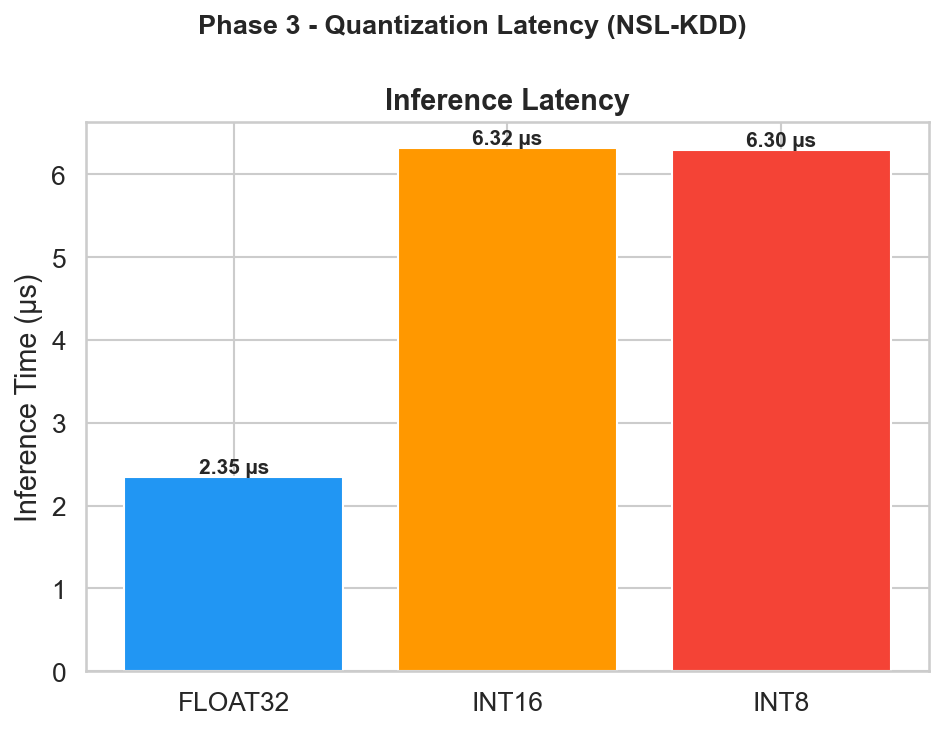
\includegraphics[width=\linewidth]{images/06c_quantization_latency.png}
    \caption{Inference latency comparison.}
  \end{subfigure}
  \caption{Quantization trade-offs for Float32, Int16, and Int8 variants.}
  \label{fig:quant_tradeoffs}
\end{figure}

% ============================================================
\section{Decision Tree Structure}
\begin{figure*}[h]
    \centering
    \includegraphics[width=\linewidth]{images/03_tree_structure_can.png}
    \caption{Trained TinyDecisionTree for the Satellite CAN IDS. Depth~5, 39~nodes, 20~leaves. Node color indicates class majority (blue = normal, orange = attack); numbers show Gini impurity, sample count, and class distribution. The tree is exported verbatim as static C arrays; inference traverses at most 5 comparisons per frame.}
    \label{fig:tree_structure}
\end{figure*}

\begin{figure}[t]
    \centering
    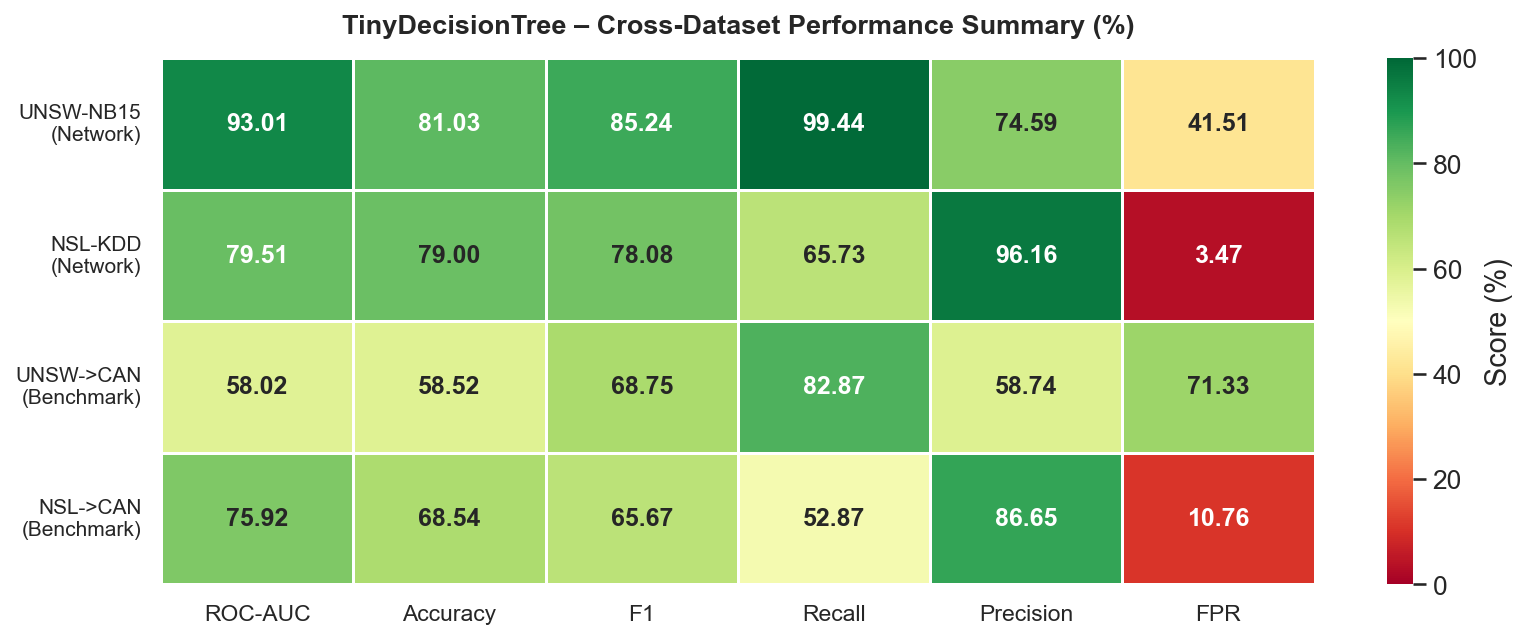
\includegraphics[width=\linewidth]{images/08_cross_dataset_heatmap.png}
    \caption{TinyDecisionTree performance heatmap across evaluation domains. Metrics are in percent; FPR is inverted (higher = lower FPR). The satellite CAN IDS achieves the strongest overall profile.}
    \label{fig:heatmap_summary}
\end{figure}